%EXPLICAR OS ELEMENTOS DE PROBABILIDADE COM OS QUAIS ESTAMOS LIDANDO:%
%QUEM S\~{A}O AS VARI\'{A}VEIS ALEAT\'{O}RIAS E COMO VAMOS DOMIN\'{A}-LAS NO TEXTO,
%COMENTAR QUE ESTAMOS TRATANDO COM VARI\'{A}VEIS DISCRETAS, COMO VAMOS IDENTIFICAR AS PROBABILIDADES,$\ldots$
%
%EXPLICAR O QUE OS \'{I}NDICES REPResentam, e as varii\'{a}veis.
%
%EXPLICAR OS TERMOS $\omega$ e $\phi$. $\omega$ \'{E} para os pesos, e $\phi$ para o bias de cada unidade.
%
%EXPLICAR MINHA NOTA\c{C}\~{A}O sobre o sobre-escrito entre par\^{e}nteses!!!
%

In this chapter will expose the theory behind the Boltzmann Machine.
A few considerations regarding the notations that will be adopt in this text is required before stepping forward into the main content.

A single random variables are denoted by $\mathrm{x}$ and $\mathrm{y}$.
A vector of random variables of size $n$ is represented by $\mathbf{x} = (\mathrm{x}_{1}, \mathrm{x}_{2}, \dots, \mathrm{x}_{n})$, where each $\mathrm{x}_{i}$, $i \in \{1, 2, \dots, n\}$, represents a single variable. 
Analagously a vector of random variables of size $m$ is represented by $\mathbf{y}$.

In a discrete scenario, the probability $P(\mathrm{x}_{i} = x_{i})$ represents the probability that a random variable $\mathrm{x}_{i}$ assumes value $x_{i}$.


The first section of this chapter introduces the Hopfield Network. We believe Hopfield Networks is an important theoretical basis before Boltzmann Machines, as some authors refer to the last as a generalization of the first one. This theory is mainly based on \cite{bib:hertz1991}. Following, the second section introduces the Boltzmann Machine; most of the theory is also base on \cite{bib:hertz1991} and [GOODFELLOW].


We begin this chapter by briefly introducing the Hopfield Network.
The reason is because the Boltzmann Machine is a generalization of the Hopfield Network.
In Hopfield Networks units are deterministic while, in Boltzmann Machines, units are stochastic.


\section{Hopfield Networks}%
\label{ch:bm:hopfield}%

Hopfield networks are a simple neural network architecture, often referred to as an associative memory network~\cite{bib:hertz1991}.
Each unit $\mathrm{x}_{i}$ in a Hopfield network is a binary unit that can assume a value $x_{i} \in \{0, 1\}$.
As~\citeonline{bib:geron2017} mentioned, this kind of network is first taught a few patterns, and then when exposed to new patterns it will output the closest learned pattern.
In the context of image recognition, we consider that each pixel of a binary image maps to one neuron of the network, then the previous statement can be read as the case where the training set contains images of characters, for instance, which are the stored memories of the network; if a new image of a character is presented, the network will recall from the memory the closest character.

In Figure~\ref{fig:hopfield-diagram}, we can see a diagram of the architecture of a Hopfield network.
It is a fully connected graph of binary units, which means that each unit is connected to every other unit of the network.
It is a different network arrangement compared to perceptron, for instance, where there is no back-coupling~\cite{bib:hopfield1982}.
\begin{figure}[h!tbp]{\textwidth}
    \centering
    \caption{Boltzmann machine diagram.}
    \label{fig:bm-diagram}
    
    \tikzstyle{visible} = [draw, circle, fill=white]
    \tikzstyle{hidden} = [draw, circle, fill=gray!30]
    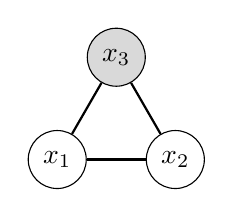
\begin{tikzpicture}
        \node[style=visible] (a) at (0, 0) {$x_{1}$};
        \node[style=visible] (b) at +(0: 1.5) {$x_{2}$};
        \node[style=hidden] (c) at + (60: 1.5) {$x_{3}$};
        \foreach \from/\to in {a/b, b/c, c/a}
            \draw [thick] (\from) -- (\to);   
    \end{tikzpicture}
  	\legend{Gray circles represent the hidden units of the Boltzmann Machine, while the white circles are the visible units.}
    % \source{\license}
\end{figure}

Hopfield network is an energy-based model, because there is a global energy function associated to the network.
This global energy function evolves to a low-energy state during training phase, i.e., the network connections between units are modified so that the energy decreases; the less energy, the better.
When connections $\omega$ between units, also know as weights or \textit{synaptic strenght}, are symmetrical, i.e., $\omega_{ij} = \omega_{ji}$, where the subscript identify the connection between unit $i$ and $j$, then~\citeonline{bib:hopfield1982} presented that the energy function is given by
\begin{equation}\label{eq:hopfield-energy}
  H(\mathbf{x}) = -\frac{1}{2}\sum_{i} \sum_{j} \omega_{ij} x_{i} x_{j} - \sum_{i} \phi_{i} x_{i},
\end{equation}
where $\mathbf{x} = (x_{1}, x_{2}, \dots, x_{n})$ is the vector of binary values that each unit of the network has for in a particular state, and $n$ is the number of units in the network.
Equation~(\ref{eq:hopfield-energy}) shows that the energy is the sum of many contributions.
Each contribution depends on one connection weight $\omega_{ij}$ and the binary state in which each neuron is, $x_{i}$ and $x_{j}$, first term of the equation.
And the second term only involves the state of each individual unit weighted by bias $\phi_{i}$.

If we want to store a pattern in a Hopfield network, we require the network to learn the right connection between units, so that this pattern can be accessed later on. To compute de proper connection in a network with $N$ units, we can proceed as follows
\begin{equation}
  \label{eq:hopfield-learn}
  \omega_{ij} = \frac{1}{N} x_{i} x_{j}.
\end{equation}

The quadratic energy function, equation~(\ref{eq:hopfield-energy}), makes it possible for each unit to compute locally how its state affects the global energy, in another words, how each unit affects the global energy when its state is changed.
Define the energy gap $\Delta H_{i}$ for a unit $x_{i}$, as the measure of the global energy function difference when the unit $x_{i}$ has its state changed.
\begin{equation}
  \label{eq:hopfield-energy-gap}
  \Delta H_{i} = H(x_{i} = 0) - H(x_{i} = 1) = \sum_{j} \omega_{ij} x_{j} + \phi_{i},
\end{equation}
the energy gap equation can also be read as the difference between the energy when $x_{i}$ is off, $x_{i} = 0$, and the energy when $x_{i}$ is on, $x_{i} = 1$.
In addition, it can also be computed by differenciating the energy function $H$, equation~(\ref{eq:hopfield-energy}). [Derivation to be added to appendix].
The Hopfield network will go down hill in this global energy.
To find the energy minimum, start from a random state, update each unit one at a time in random order. Update each unit to whichever of its two states gives the lowest global energy.

According to~\citeonline{bib:hopfield1982}, memories can be seen as energy minima.
Furthermore, by just knowing some parts of an energy minima, its possible to access that memory.
An interesting analogy, is that Hopfield networks are like reconstructing a dinosaur from a few bones.

%FALTA COLOCAR A REGRA DE ATUALIZACAO DOS PESOS\@! PARA MOSTRAR COMO AS MEMORIAS SAO ARMAZENADAS.\@


\section{Boltzmann Machines}%
\label{ch:bm:bm}%

Boltzmann Machines are a type of stochastic neural networks where the connections between units, which are described by $\omega$, are symmetrical, i.e., $\omega_{ij} = \omega_{ji}$~\cite{bib:hertz1991}. 
This kind of stochastic neural networks are capable of learning internal representation and to model an input distribution. 
Boltzmann Machines were named after the Boltzmann distribution. 
Due to its stochatics behaviour, the probability of the state of the system to be found in a certain configuration is given by previous mentioned distribution~\cite{bib:hertz1991}. 
According to~\cite{bib:montufar2018}, Boltzmann machines can be seen as an extension of Hopfield networks to include hidden units and units with a stochastic behaviour.

Boltzmann Machines have two kind of units $\mathrm{x}_{i}$: the visible and hidden units. 
The visible units are linked to the external world and they correspond to the components of an observation, where data is input. On the other hand, the hidden units do not have any connection outside of the network and they model the dependencies between the components of the observations~\cite{bib:fischer2012}, i.e., they are responsible for finding the data relation from the input. 
In Boltzmann machines, there is no connection restriction, this means that every unit, visible or hidden, can be connected to every other unit as in a complete graph, this pattern is not mandatory as some of the connections may not exists depending on the network layout. 
Regardless of how the connections are, if there is a connection bewteen two units, this connection is symmetric. 
Training a Boltzmann Machines means finding the right connections $\omega_{ij}$ between the units.

In Figure~\ref{fig:bm-diagram}, we have a diagram of a Boltzmann machine layout. 
We can see that each unit is connected to every other unit in the network regardless of it being a visible or hidden unit.
\begin{figure}[h!tbp]{\textwidth}
  \centering
  \caption{Boltzmann machine diagram.}%
  \label{fig:bm-diagram}%
  \tikzstyle{visible} = [draw, circle, fill=white]
  \tikzstyle{hidden} = [draw, circle, fill=gray!30]
  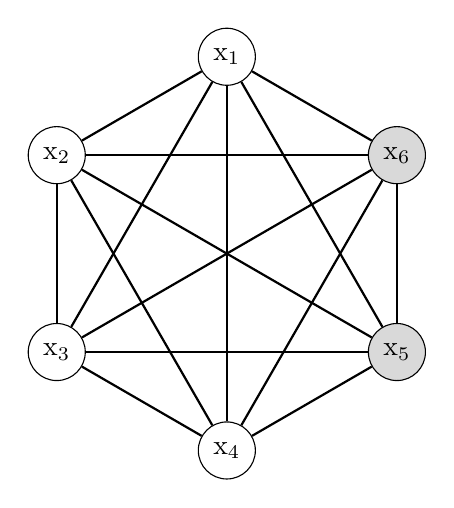
\begin{tikzpicture}
    \node[style=visible] (a) at (0, 2.5) {$\mathrm{x}_{1}$};
    % \node[style=visible] (b) at +(0: 1.5) {$\mathrm{x}_{2}$};
    % \node[style=hidden] (c) at + (60: 1.5) {$\mathrm{x}_{3}$};
    \node[style=visible] (b) at (-2.16, 1.25) {$\mathrm{x}_{2}$};
    \node[style=visible] (c) at (-2.16, -1.25) {$\mathrm{x}_{3}$};
    \node[style=visible] (d) at (0, -2.5) {$\mathrm{x}_{4}$};
    \node[style=hidden]  (e) at (2.16, -1.25) {$\mathrm{x}_{5}$};
    \node[style=hidden]  (f) at (2.16, 1.25) {$\mathrm{x}_{6}$};
    \foreach \from/\to in {a/b, a/c, a/d, a/e, a/f, b/c, b/d, b/e, b/f, c/d, c/e, c/f, d/e, d/f, e/f}
      \draw [thick] (\from) -- (\to);   
  \end{tikzpicture}
  \legend{Gray circles represent the hidden units of the Boltzmann Machine, while the white circles are the visible units.}
  \source{Author.}
\end{figure}


Stochastics units $\mathrm{x}_{i}$ compose the Boltzmann machine. 
Stochastics units are random variables $\mathrm{x}$ that can assume a binary value with a certain probability.
We will consider that a random variable $\mathrm{x}_{i}$ can assume a value of $x_{i} = 1$ with probability $g(h_{i})$, and $x_{i} = 0$, otherwise, i.e.,
\begin{equation}
  \label{eq:stochastic-unit-values}
  x_{i} =
    \begin{cases}
      1 \; \text{with probability} \; g(h_{i}) \\
      0 \; \text{with probability} \; 1 - g(h_{i})
    \end{cases},
\end{equation}
where the probability $g(h_{i})$ is given by
\begin{equation}
  \label{eq:stochastic-unit-prob}
  g(h_{i}) = \frac{1}{1 + e^{-2 \beta h_{i}}},
\end{equation}
and
\begin{equation}
  \label{eq:stochastic-unit-input}
  h_{i} = \sum_{j}\omega_{ij}x_{j} + \phi_{i},
\end{equation}
equation~(\ref{eq:stochastic-unit-input}) stands for the input a unit $x_{i}$ receives.

Likewise the Hopfield network, due to the symmetrical connections, there is an energy function which is also given by equation~(\ref{eq:hopfield-energy}). This energy function has minimum when there is a stable state characterised by
\begin{equation}
  \label{eq:stochastic-stable-state}
  x_{i} = step(h_{i}).
\end{equation}

For stochastics neural networks the probability $P$ of finding the system in a given state $\mathbf{x}$ after the equilibrium is reached is
\begin{equation}
  \label{eq:stochastic-prob}
  P(\mathbf{x}) = \frac{1}{Z} e^{-\beta H(\mathbf{x})},
\end{equation}
where
\begin{equation}
  \label{eq:stochastic-z}
  Z = \sum_{\mathbf{x}'} e^{-\beta H(\mathbf{x}')}
\end{equation}
is the partition function. The vector $\mathrm{\mathbf{x}}$ represents the state in which the units of the network are, for instance, the following state, in a 3 units stochastic network, $\mathrm{\mathbf{x}} = (x_{1}, x_{2}, x_{3}) = (1, 0, 1)$.

%The learning process of a Boltzmann Machine consists in ajusting the connections $\omega_{ij}$ in such a way that the state of the visible units have a particular desired probability distribution.
Now let us consider the Boltzmann machine case where there are two kinds of units, i.e., the visible and the hidden units. 
Let us identify the state of the visible units by an index $v$ and the state of the hidden units by an index $h$. 
Considering a particular system with $N$ visible units and $K$ hidden units, the whole system have $2^{N + K}$ possibilities of states in which it can be found.

The joint probability $P_{vh}$ is the probability of finding the visible and hidden units in the states $v$ and $h$, respectively.
This probability distribution is given by the Boltzmann distribution
\begin{equation}
  \label{eq:bm-joint-prob}
  P_{vh} = \frac{1}{Z}e^{-\beta H_{vh}},
\end{equation}
where
\begin{equation}
  \label{eq:bm-z}
  Z = \sum_{u} \sum_{k} e^{-\beta H_{uk}},
\end{equation}
and
\begin{equation}
  \label{eq:bm-energy-function}
  H_{vh} = - \frac{1}{2} \sum_{i} \sum_{j} \omega_{ij} x^{(vh)}_{i} x^{(vh)}_{j} - \sum_{i} \phi_{i} x^{(vh)}_{i}.
\end{equation}

Equations~(\ref{eq:bm-joint-prob}),~(\ref{eq:bm-z}) and~(\ref{eq:bm-energy-function}) are ajustments to equations~(\ref{eq:stochastic-prob}),~(\ref{eq:stochastic-z}) and~(\ref{eq:hopfield-energy}), respectively, where now the different kind of units state is taken into consideration. 
In equation~(\ref{eq:bm-z}), the indexes $u$ and $k$ refer to visible and hidden units states, respectively, different indexes are used to avoid bewilderment.

As previously mentioned, the problem a Boltzmann Machine is trying to solve is determining the connections $\omega_{ij}$ between units such that the visible units have a certain probability distribution. 
In order to do that, we need to find the marginal probability of the state $v$ in which the visible units are found regardless of the state $h$ of the hidden units. The marginal probability $P_{v}$ is given by
\begin{equation}
  \label{eq:bm-marginal-prob}
  P_{v} = \sum_{h} P_{vh} = \sum_{h} \frac{e^{-\beta H_{vh}}}{Z}.
\end{equation}

Although we know that $P_{v}$ is a function of the connections $\omega_{ij}$, and that this is the probability of finding the visible units in the state $v$. We want the states to have a certain probability $R_{v}$, i.e., a desired probability.
This means that ideally we would like to match the empirical distribution of the data, even though we do not have access to the correct distribution, only to what the observed data has given us as an input to training the model.

One way to evaluate the difference between two probability distribution, for example, $P_{v}$ and $R_{v}$, is using the Kullback-Leibler divergence $D_{KL}(R_{v}||P_{v})$, which can also be referred to as relative entropy, $E$, which will be our cost function. 
Further comments about the Kullback-Leibler divergence can be found on appendix~\ref{app:dkl}.
%(EXPLICAR FUN\c{C}\~{A}O DE CUSTO e $D_{KL}$!!!).
\begin{equation}
  \label{eq:relative-entropy}
  E = \sum_{v} R_{v} \ln{\left(\frac{R_{v}}{P_{v}}\right)}.
\end{equation}

The relative entropy $E$ has the property of always being equal or greater than zero. 
It reaches zero only if $P_{v} = R_{v}$, which means that we are able to retrieve the exactly desired probability distribution at the visible units from the input data. 
We have to minimise $E$ using the gradient descent~\cite{bib:hertz1991}, relative to the weights $\omega_{ij}$ and the bias $\phi_{i}$, 
\begin{equation}
  \label{eq:delta-omega}
  \Delta \omega_{ij} = -\eta \frac{\partial E}{\partial \omega_{ij}},
\end{equation}
and
\begin{equation}
  \label{eq:delta-phi}
  \Delta \phi_{i} = -\eta \frac{\partial E}{\partial \phi_{i}},
\end{equation}
where
\begin{equation}
  \label{eq:relative-entropy-expansion}
  \begin{split}
    E & = \sum_{v} R_{v} \ln{\left(\frac{R_{v}}{P_{v}}\right)} \\
      & = \sum_{v} \left[ \ln{(R_{v})} - \ln{(P_{v})} \right].
  \end{split}
\end{equation}

In the following steps, we present the derivation of the gradient descent, based on the derivation in~\cite{bib:hertz1991}
\begin{equation}
  \label{eq:relative-entropy-grad-step1}
  \begin{split}
    \Delta \omega_{ij} & = - \eta \frac{\partial E}{\partial \omega_{ij}} \\
                  & = - \eta \frac{\partial}{\partial \omega_{ij}} \left[ \sum_{v} R_{v} \left( \ln{(R_{v})} - \ln{(P_{v})} \right) \right] \\
                  & = \eta \frac{\partial}{\partial \omega_{ij}} \left[ \sum_{v} R_{v} \ln{(P_{v})} \right] \\
                  & = \eta \sum_{v} R_{v} \frac{\partial}{\partial \omega_{ij}} \left[ \ln{(P_{v})} \right] \\
                  \Rightarrow & \Delta \omega_{ij} = \eta \sum_{v} \frac{R_{v}}{P_{v}} \frac{\partial P_{v}}{\partial \omega_{ij}}.
  \end{split}
\end{equation}

To continue with the computation of $\Delta \omega_{ij}$, we have to find the derivative of $\partial P_{v}/\partial \omega_{ij}$, from the marginal probability, equation~(\ref{eq:bm-marginal-prob}),
\begin{equation}
  \label{eq:bm-marginal-prob-expansion}
  P_{v} = \frac{\sum_{h} e^{-\beta H_{vh}}}{\sum_{u} \sum_{k} e^{-\beta H_{u k}}},
\end{equation}
thus the derivative of $P_{v}$ follows
\begin{equation}
  \label{eq:bm-marginal-prob-grad}
  \begin{split}
    \frac{\partial P_{v}}{\partial \omega_{ij}} & = \frac{\partial}{\partial \omega_{ij}} \left[ \frac{\sum_{h} e^{-\beta H_{vh}}}{\sum_{u} \sum_{k} e^{-\beta H_{u k}}} \right] \\
    & = \frac{1}{\sum_{u} \sum_{k} e^{-\beta H_{u k}}} \sum_{h} (-\beta) e^{-\beta H_{vh}} \frac{\partial H_{vh}}{\partial \omega_{ij}} \\
    & - \sum_{h} e^{-\beta H_{vh}} \frac{1}{{\left( \sum_{u} \sum_{k} e^{-\beta H_{u k}} \right)}^{2}} \sum_{u} \sum_{k} e^{-\beta H_{u k}} (-\beta) \frac{\partial H_{u k}}{\partial \omega_{ij}}.
  \end{split}
\end{equation}

Following equation~(\ref{eq:bm-marginal-prob-grad}), we need to compute the term $\partial H_{vh}/\partial \omega_{ij}$,
\begin{equation}
  \label{eq:bm-energy-grad-step1}
  \begin{split}
      \frac{\partial H_{vh}}{\partial \omega_{ij}} & = \frac{\partial}{\partial \omega_{ij}} \left[- \frac{1}{2} \sum_{m} \sum_{n} \omega_{mn} x^{(vh)}_{m} x^{(vh)}_{n} - \sum_{m} \phi_{mm} x^{(vh)}_{m} \right] \\
                                                   & = \frac{\partial}{\partial \omega_{ij}} \left[- \frac{1}{2} \sum_{m \neq i,j} \sum_{n \neq i,j} \omega_{mn} x^{(vh)}_{m} x^{(vh)}_{n} - \frac{1}{2} \omega_{ij} x^{(vh)}_{i} x^{(vh)}_{j} - \frac{1}{2} \omega_{ji} x^{(vh)}_{j} x^{(vh)}_{i} - \sum_{m} \phi_{m} x^{(vh)}_{m} \right],
  \end{split}
\end{equation}
as the connections between units are symmetric, i.e., $\omega_{ij} = \omega_{ji}$, we can simplify equation~(\ref{eq:bm-energy-grad-step1}),
\textbf{RRUMAR OS ÍNDICES!!!}
\begin{equation}
  \label{eq:bm-energy-grad-final}
  \begin{split}
    \frac{\partial H_{vh}}{\partial \omega_{ij}} & = \frac{\partial}{\partial \omega_{ij}} \left[- \frac{1}{2} \sum_{m \neq i,j} \sum_{n \neq i,j} \omega_{mn} x^{(vh)}_{m} x^{(vh)}_{n} - \omega_{ij} x^{(vh)}_{i} x^{(vh)}_{j} - \sum_{m} \phi_{m} x^{(vh)}_{m} \right] \\
    & = \frac{\partial}{\partial \omega_{ij}} \left[- \frac{1}{2} \sum_{m \neq i,j} \sum_{n \neq i,j} \omega_{mn} x^{(vh)}_{m} x^{(vh)}_{n} \right] + \frac{\partial}{\partial \omega_{ij}} \left[- \omega_{ij} x^{(vh)}_{i} x^{(vh)}_{j} \right] + \frac{\partial}{\partial \omega_{ij}} \left[- \sum_{m} \phi_{m} x^{(vh)}_{m} \right] \\
    \Rightarrow & \frac{\partial H_{vh}}{\partial \omega_{ij}} = - x^{(vh)}_{i} x^{(vh)}_{j}.
  \end{split}
\end{equation}

Analagous to $\partial H_{vh}/\partial \omega_{ij}$, we have the derivative of $H_{uk}$ which is
\begin{equation}
  \label{eq:bm-energy-grad-final2}
  \frac{\partial H_{uk}}{\partial \omega_{ij}} = - x^{(uk)}_{i} x^{(uk)}_{j}.
\end{equation}

Going back to equation~(\ref{eq:bm-marginal-prob-grad}), we can replace the derivatives of $H$, and solve the derivative of the marginal probability $P_{v}$,
\begin{equation}
  \label{eq:bm-marginal-prob-grad-final}
  \begin{split}
    \frac{\partial P_{v}}{\partial \omega_{ij}} & = \frac{1}{Z} \sum_{h} e^{-\beta H_{vh}} (-\beta) (-x^{(vh)}_{i} x^{(vh)}_{j}) - \frac{1}{Z^{2}} \sum_{h} e^{-\beta H_{vh}} \sum_{u} \sum_{k} e^{-\beta H_{uk}} (-\beta) (-x^{(uk)}_{i} x^{(uk)}_{j}) \\
    & = \beta \left[ \sum_{h} \frac{e^{-\beta H_{vh}}}{Z} x^{(vh)}_{i} x^{(vh)}_{j} - \sum_{h} \frac{e^{-\beta H_{vh}}}{Z} \sum_{u} \sum_{k} \frac{e^{-\beta H_{uk}}}{Z} x^{(uk)}_{i} x^{(uk)}_{j}  \right] \\
    & = \beta \left[ \sum_{h} P_{vh} x^{(vh)}_{i} x^{(vh)}_{j} - P_{v} \sum_{u} \sum_{k} P_{uk} x^{(uk)}_{i} x^{(uk)}_{j} \right] \\
    \Rightarrow & \frac{\partial P_{v}}{\partial \omega_{ij}} = \beta \left[ \sum_{h} P_{vh} x^{(vh)}_{i} x^{(vh)}_{j} - P_{v} \langle x_{i} x_{j} \rangle  \right].
  \end{split}
\end{equation}

Given the derivative of $P_{v}$ in relation to $\omega_{ij}$, we can compute the learning term $\Delta \omega_{ij}$, from equation~(\ref{eq:relative-entropy-grad-step1}),
\begin{equation}
  \label{eq:delta-omega-final}
  \begin{split}
    \Delta \omega_{ij} & = \eta \sum_{v} \frac{R_{v}}{P_{v}} \beta \left[ \sum_{h} P_{vh} x^{(vh)}_{i} x^{(vh)}_{j} - P_{v} \langle x_{i} x_{j} \rangle \right]  \\
    & = \eta \beta \left[ \sum_{v} \sum_{h} \frac{R_{v}}{P_{v}} P_{vh} x^{(vh)}_{i} x^{(vh)}_{j} - \sum_{v} \frac{R_{v}}{P_{v}} P_{v} \langle x_{i} x_{j} \rangle \right] \\
    & = \eta \beta \left[ \sum_{v} \sum_{h} R_{v} \frac{P_{vh}}{P_{v}} x^{(vh)}_{i} x^{(vh)}_{j} - \sum_{v} R_{v} \langle x_{i} x_{j} \rangle \right] \\
    & = \eta \beta \left[ \sum_{v} \sum_{h} R_{v} P_{h|v} x^{(vh)}_{i} x^{(vh)}_{j} - \langle x_{i} x_{j} \rangle \right].
  \end{split}
\end{equation}

In the above derivation, we have used the following relations,
\begin{equation}
  \label{eq:conditional-prob1}
  P_{h|v} = \frac{P_{vh}}{P_{v}},
\end{equation}
which is the conditional probability equation.
In our scenario this equation means that the probability distribution of the hidden units in state $h$ given the state $v$ of the visible units is the joint probability distribution of both states, $v$ and $h$, divided by the marginal probability distribution of the visible units in state $v$.

The second term in equation~(\ref{eq:delta-omega-final}), is the average of units $i$ and $j$ over all combinations of states $v$ and $h$ of the system.
In other words, we would have to compute all possible combination of states of visible and hidden units, $v$ and $h$, and then average over the specific units $i$ and $j$.

The first term can be simplified by
\begin{equation}
  \label{eq:clamped-term}
  \sum_{v} R_{v} \sum_{h} P_{h|v} x^{(vh)}_{i} x^{(vh)}_{j} = \sum_{v} R_{v} \langle x_{i} x_{j} \rangle^{(v)} = \langle \langle x_{i} x_{j} \rangle^{(v)} \rangle,
\end{equation}
which is the average value according to the probability distribution $R_{v}$ of the correlation between variables $x_{i}$ and $x_{j}$ when the visibles units are fixed at state $v$.

Then equation~(\ref{eq:delta-omega-final}) becomes
\begin{equation}
  \label{eq:delta-omega-final2}
  \Delta \omega_{ij} = \eta \beta \left[ \langle \langle x_{i} x_{j} \rangle^{(v)} \rangle_{clamped} - \langle x_{i} x_{j} \rangle_{free} \right],
\end{equation}
it is important to notice that the subscripts \textit{clamped} means that we have to fix a certain $v$ state on the visible units otherwise the second term in the equation does not have a reference to whom it should be trying to match.
On the other hand, the subscript \textit{free} identify the case where the variables are allowed to vary freely without any restriction~\cite{bib:duda2000}. When the first and the second terms are equal, i.e., $\langle \langle x_{i} x_{j} \rangle^{(v)} \rangle_{clamped} = \langle x_{i} x_{j} \rangle_{free}$, the update in the weight is zero, $\Delta \omega_{ij} = 0$, thus the desired value of that connection is obtained.
